\chapter{近存计算架构中的矩阵向量乘硬件设计}
本章主要介绍借助近存计算模拟器的修改硬件,优化矩阵向量乘的设计。第一小节是对上一章提出的三个软件算法的性能分析。之后介绍新增融合查表加法指令对矩阵向量乘的优化手段。然后详细介绍通过增加向量单元和指令,向量化计算矩阵向量乘的设计和算法。最后说明上述设计实现的模拟器平台,简要介绍模拟器特性和硬件修改实现方式。

\section{软件优化性能瓶颈分析}

\begin{table}[!htbp]
    \centering
    \caption{软件优化性能分析}
    \label{BottleneckTable}
    \begin{tabular}{llll}
        \toprule
        算法 & 执行耗时& IPC & MBU \\
        \midrule
        LUT-M & 698.7\;ms & 96.96\% & 3.70\% \\
        LUT-W-C & 467.6\;ms &84.38\% & 11.66\% \\
        LUT-W-R & 298.8\;ms &76.97\% & 10.67\% \\
        \bottomrule
    \end{tabular}
\end{table}

在上一章提出了三种算法优化后,本小节对每种算法下的矩阵向量乘算子的在近存硬件上的执行情况进行了测试,分别测试其在特定规模和的矩阵和线程配置下的执行时间、周期数以及指令数。我们计算了不同算法的计算利用率(Instructions Per Cycle,IPC)和内存带宽利用率(MRAM Bandwidth Utilization,MBU)。这里MBU的计算公式为\ref{MBUEqu},MRAMRead是算子执行过程种从MRAM读取的数据(MB),ExecuteTime是算子执行时间(秒),通过此前的工作知道理论带宽大概为628MB/s\cite{BenchmarkingMutlu}),因此可以算出利用率。矩阵仍然采用的是$4096\times 4096$的FP8格式,开启16个Tasklets,在单一DPU上的测试如表\ref{BottleneckTable}所示。

\begin{equation}
    MBU=\frac{MRAM\;Read}{ExecuteTime\times 628}\times 100\%
    \label{MBUEqu}
\end{equation}

可以看到,在三种算法中,从LUT-M、LUT-W-C再到LUT-W-R,IPC是下降的,相应的MBU是上升的,这说明我们在针对WRAM的优化中通过增加MRAM的访存次数来减少WRAM的访存,可以看到执行时间在逐渐降低证明这种优化有效:LUT-M虽然MRAM的访问少但是执行时间长,通过额外访问MRAM获取一些辅助性数据或增加访问MRAM的次数提高寄存器的局部性可以有效的提升算子性能,是一种权衡(trade off)。

尽管如此,能观察到IPC的值始终在70\%以上,相应地MBU的值在10\%左右,这充分说明了UPMEM这个硬件平台的特性为计算瓶颈,与传统的冯诺依曼架构不同,UPMEM的访存带宽很快几乎不会成为瓶颈。想要进一步提升算子性能,本文认为仅仅在软件层面做算法的优化十分有限,需要着手与UPMEM硬件结构做出优化,比如为UPMEM增添额外的计算单元和算术能力以增强UPMEM的计算强度。这里将不探讨简单的硬件参数修改诸如提高主频、增加浮点单元支持硬件浮点算术计算等等,我们将结合我们的软件算法特点(LUT)去设计硬件的微架构的更改。

\section{查表和加法融合的指令设计}
在传统CPU平台上编程时,如果需要访问数组的某个元素,需要拿到数组的首地址addr和元素索引index,以及每个元素所占字节数为width,通过计算addr+index*width得到真正的内存地址然后再去访存。这种乘加的操作在编译时会做优化,假如数组是连续访问的,那么会优化指令递增地址:只有第一次访问数组需要计算乘加,后面访问只需要在地址寄存器累加上width即可。但是在上述基于查找表的算法,数组的访问往往不是连续的,无法消除乘加操作,因此这里可以设计增加一系列指令专门用于访问数组(查找表),如图\ref{LUTInst}所示,分别设计了适用于不同数据位宽的指令,如LHSI(Lookup Halfword Signed by Index),该指令接受dst寄存器、base寄存器、idx寄存器和移位立即数shift:dst寄存器是目标寄存器,base寄存器是数组的首地址,idx寄存器是数组的索引,shift指示的是元素宽度(2byte宽度是移位1位),这条指令的操作就是将idx寄存器的值左移shift位,然后与base寄存器的值相加得到地址addr并访存2个字节,将结果存入dst寄存器(符号位扩展)。这样数组的访问就可以通过这一条指令完成。

\begin{figure}[!htbp]
	\centering
    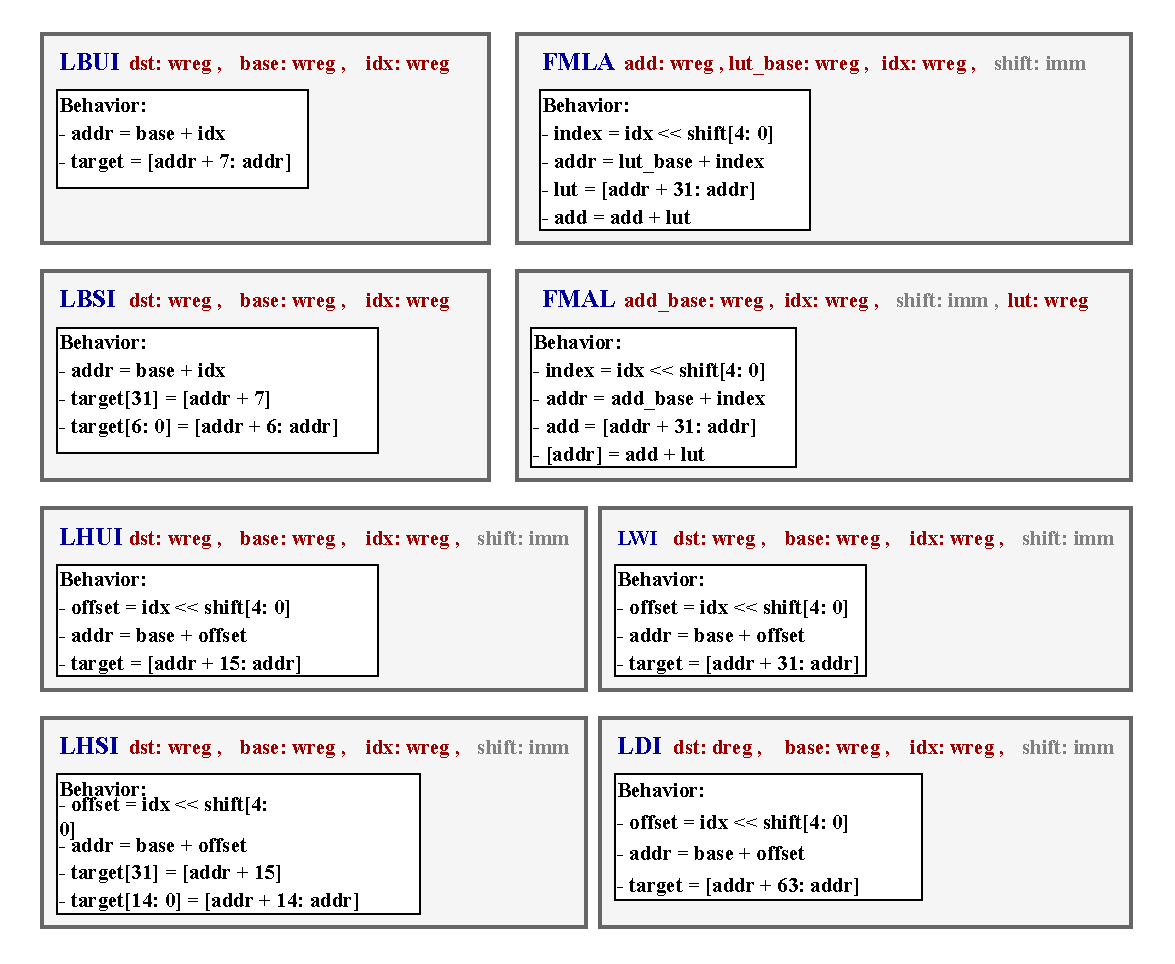
\includegraphics[width=0.9\textwidth]{figures/LUTInst.pdf}
	\caption{FLA指令集设计}
    \label{LUTInst}
\end{figure}

在矩阵乘法的计算中,能够观察到一个非常基本的操作:向量和矩阵的元素相乘再与结果向量中的元素相加,将这种乘加操作融合成为单个操作,称为融合乘加(Fused Multiply Add,FMA)操作。在许多AI加速芯片中都设计有MAC单元(Multiplier-Accumulator Unit)支持FMA操作和指令。将乘加操作融合成为一条指令的优势一方面在于能够使得指令数目减少,减少取指和译码的时间,另一方面就是能够设计专门的电路优化计算,减少消耗周期数,从而整体提高算术吞吐。因此可以基于此前的查表指令,修改UPMEM硬件支持融合查表加法指令,如图\ref{LUTInst}所示,FMLA(Fused Multiply Lookup Add)指令接受add寄存器,lut\_base寄存器,idx寄存器和移位立即数shift:add寄存器用于存放累加结果,lut\_base寄存器存放的是查找表的首地址,idx寄存则是查找表的索引,shift同样指示的是元素宽度,这条指令的操作类似此前的查表指令,先取得lut\_base[idx]结果,与add寄存器相加并累加到add中。至于FMAL(Fused Multiply Add Lookup)指令则是受armv8的LDADDA指令启发\footnote{https://developer.arm.com/documentation/dui0801/g/A64-Data-Transfer-Instructions/},专门用于解决需要频繁读写结果向量的操作,其会从内存中读取某个数进行加法运算后再存回。这一系列的指令我们称之为FLA(Fused Lookup Add)指令集。

\begin{figure}[htbp!]
	\centering
	\subfigure[LUT-M算法]{
		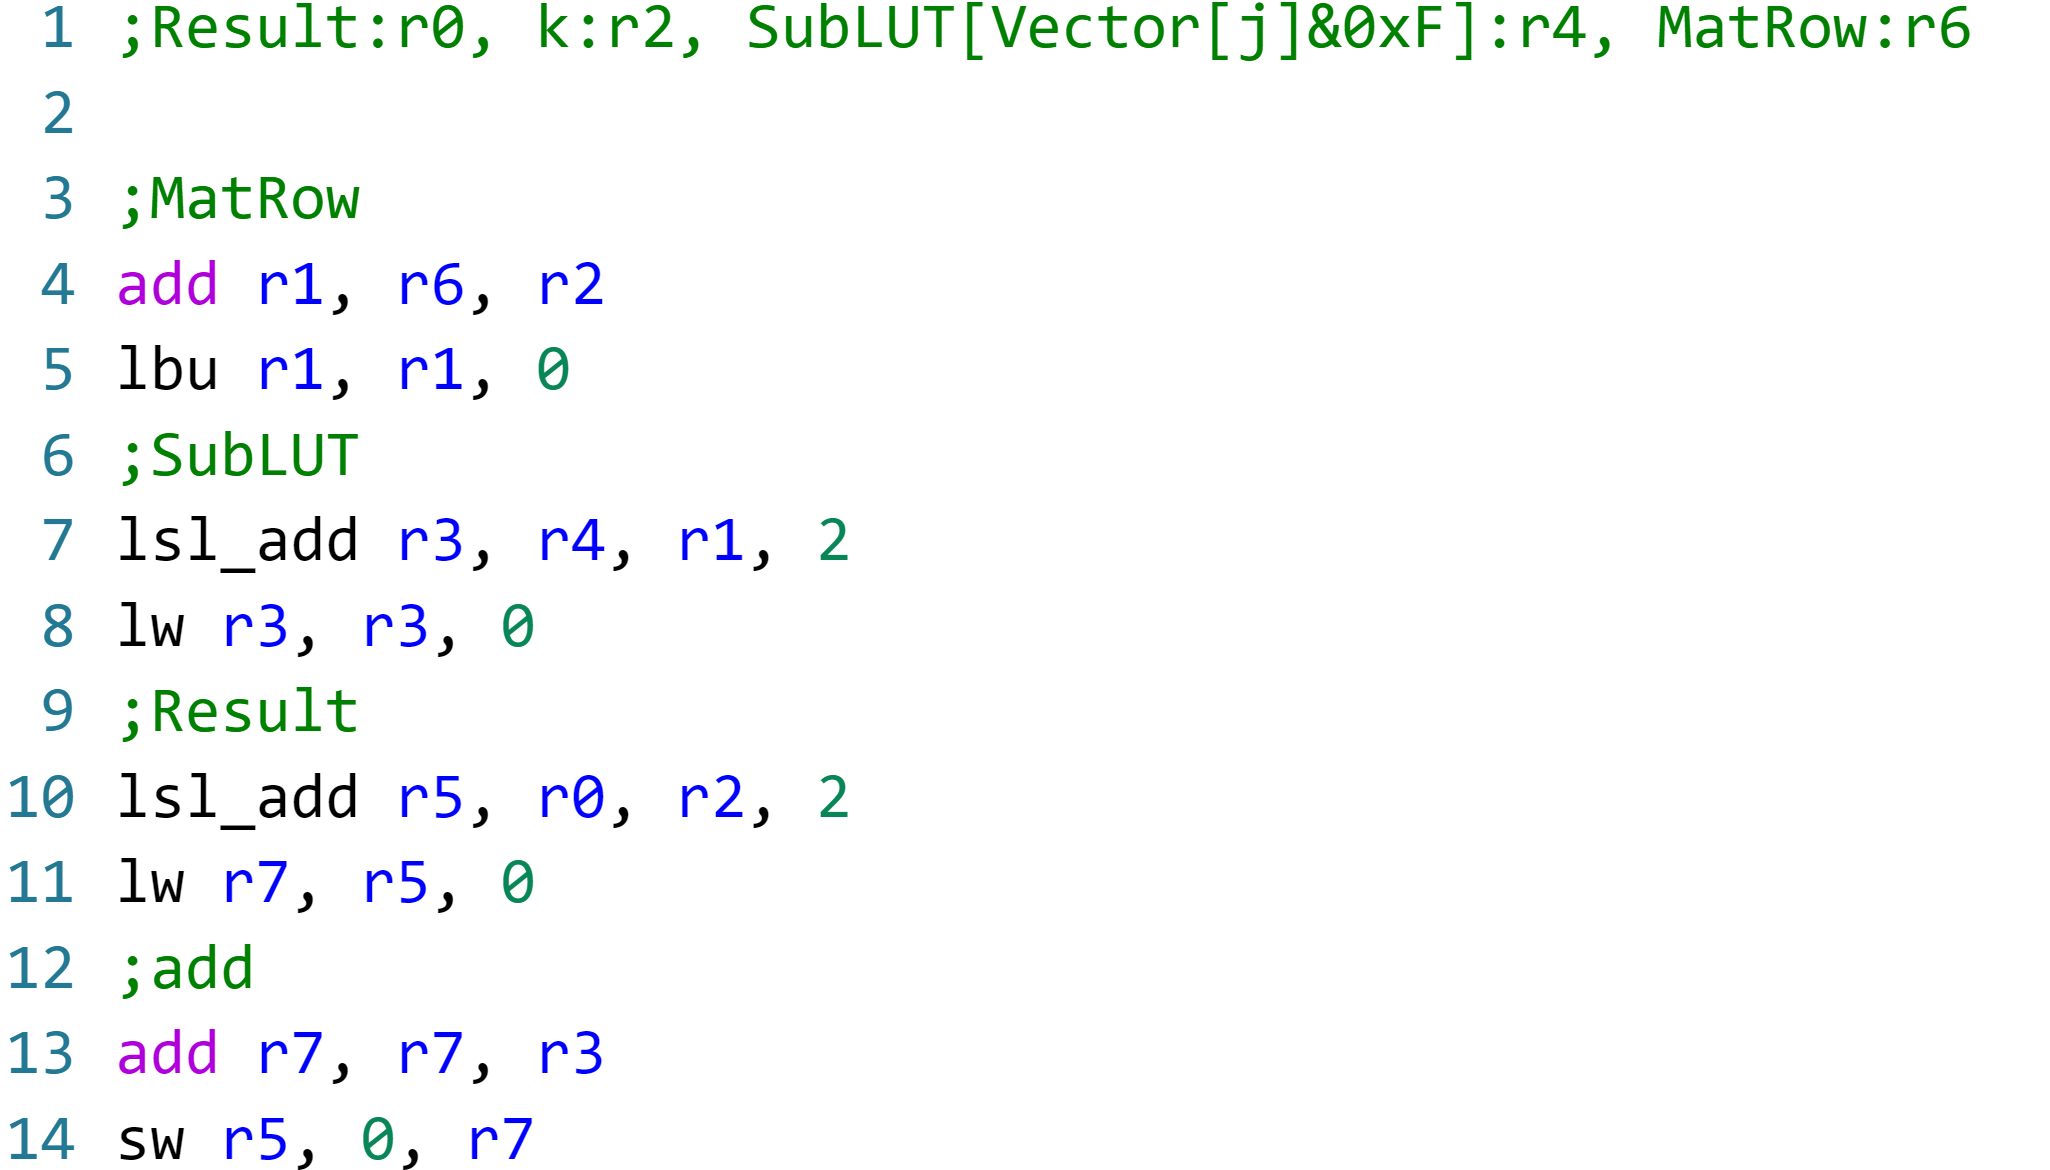
\includegraphics[width=0.3\linewidth]{figures/asm1.png}
		\label{LUTInstAsm:LUT-M}}
	\subfigure[LUT-W-R算法]{
		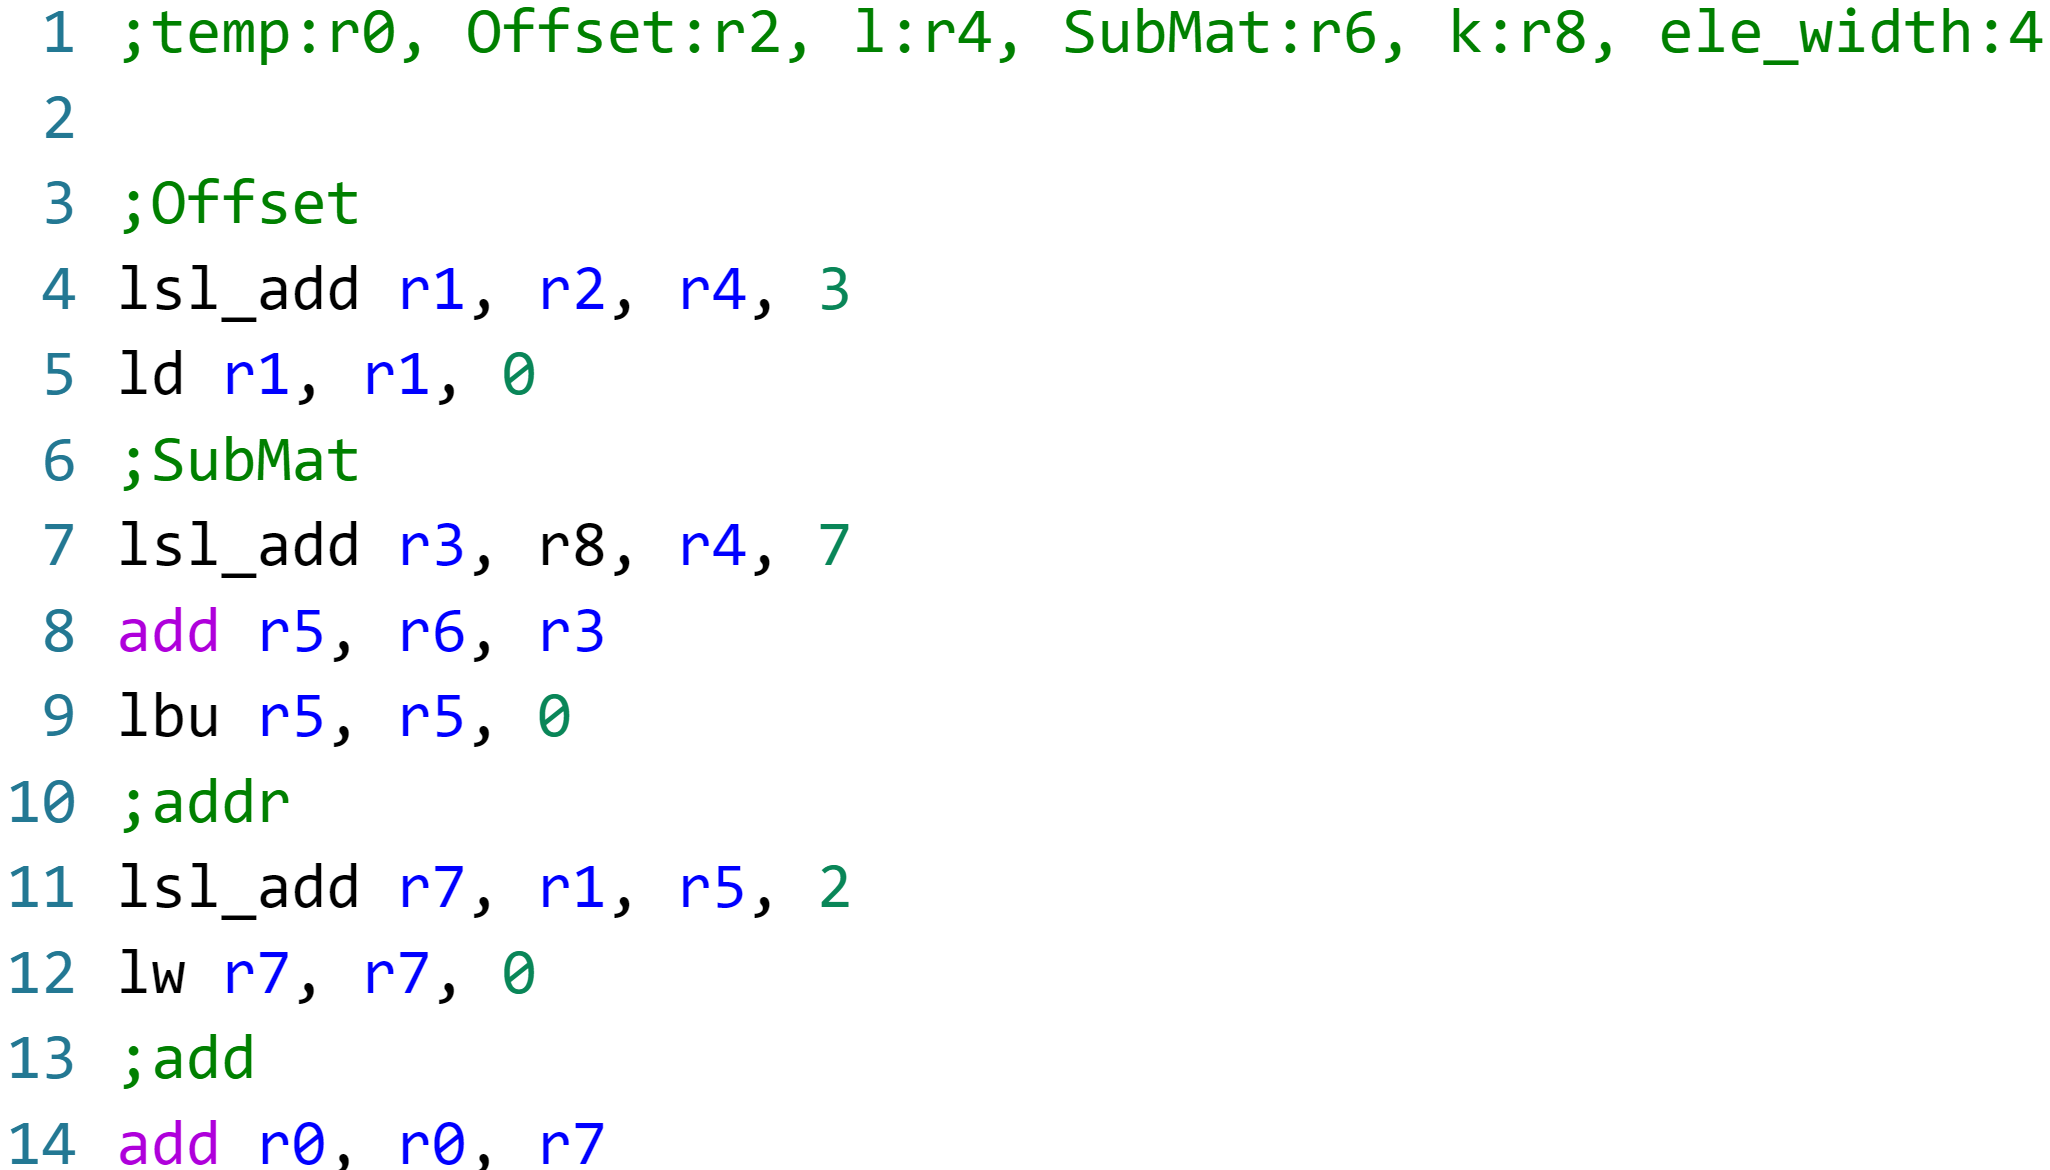
\includegraphics[width=0.3\linewidth]{figures/asm2.png}
        \label{LUTInstAsm:LUT-W-R}}
    \subfigure[LUT-W-C算法]{
        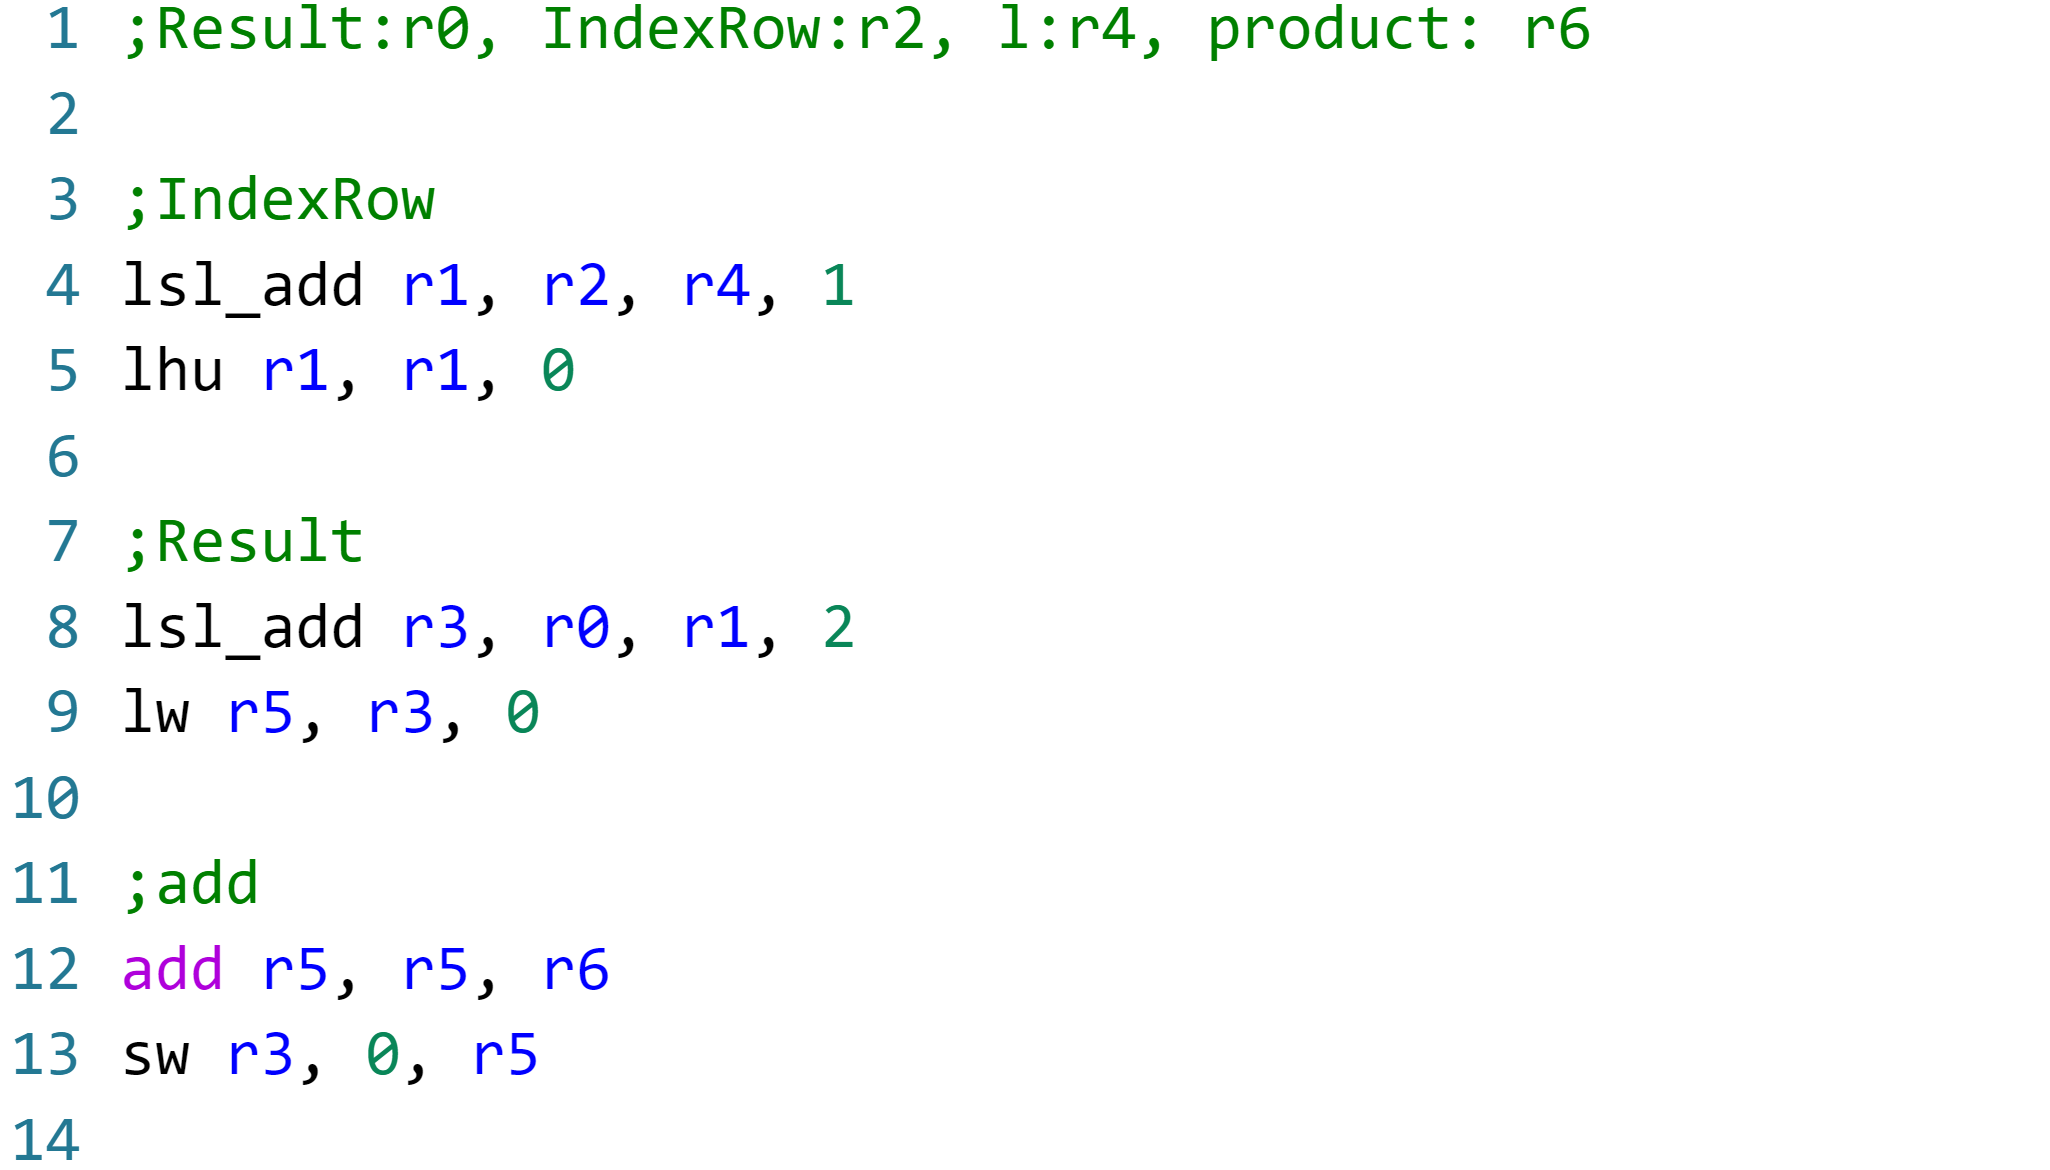
\includegraphics[width=0.3\linewidth]{figures/asm3.png}
        \label{LUTInstAsm:LUT-W-C}}
    \\
    \subfigure[LUT-M算法优化]{
        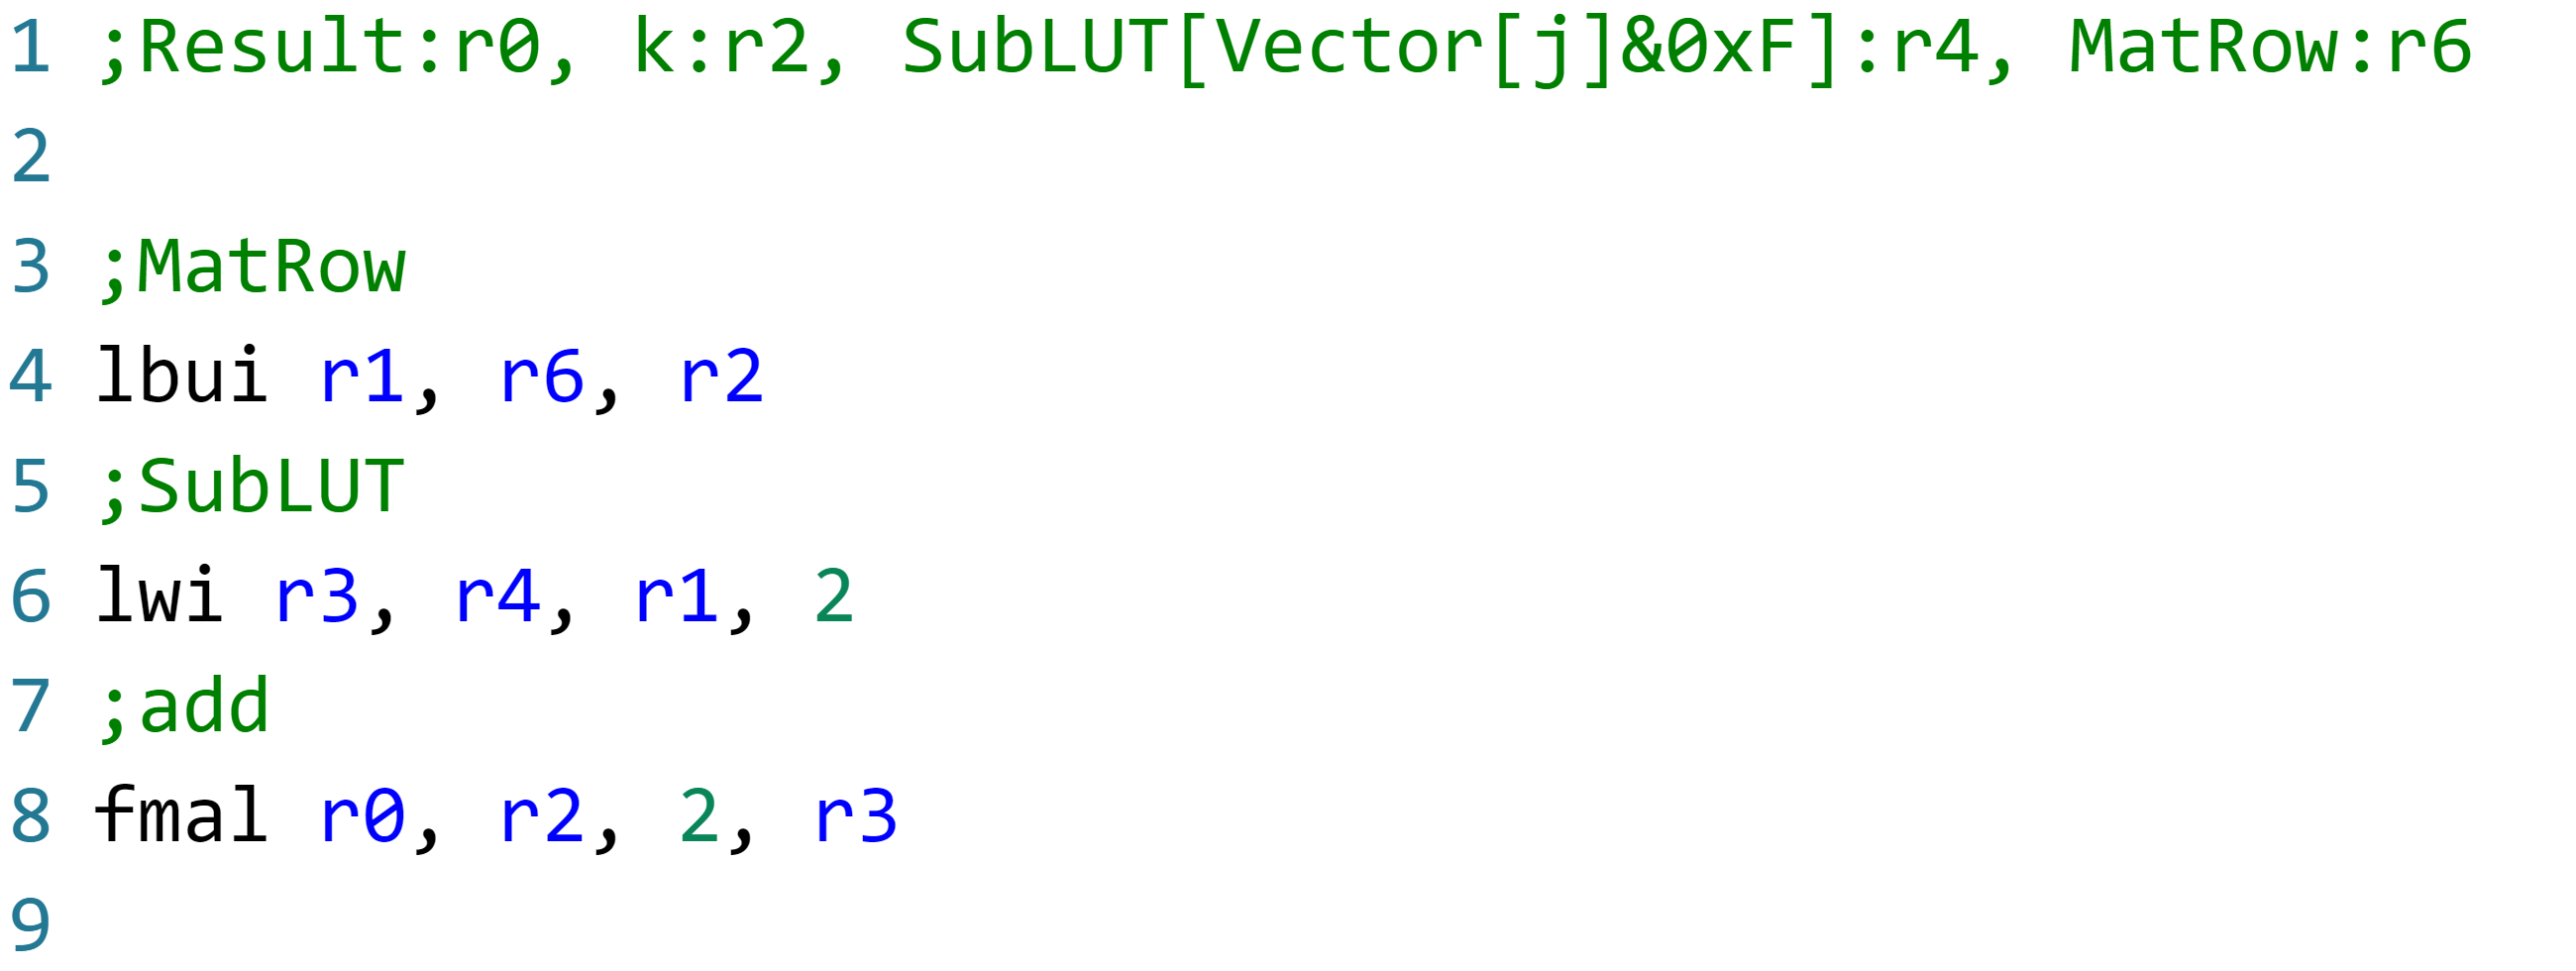
\includegraphics[width=0.3\linewidth]{figures/asm1-opt.png}
        \label{LUTInstAsm:LUT-M-opt}}
    \subfigure[LUT-W-R算法优化]{
        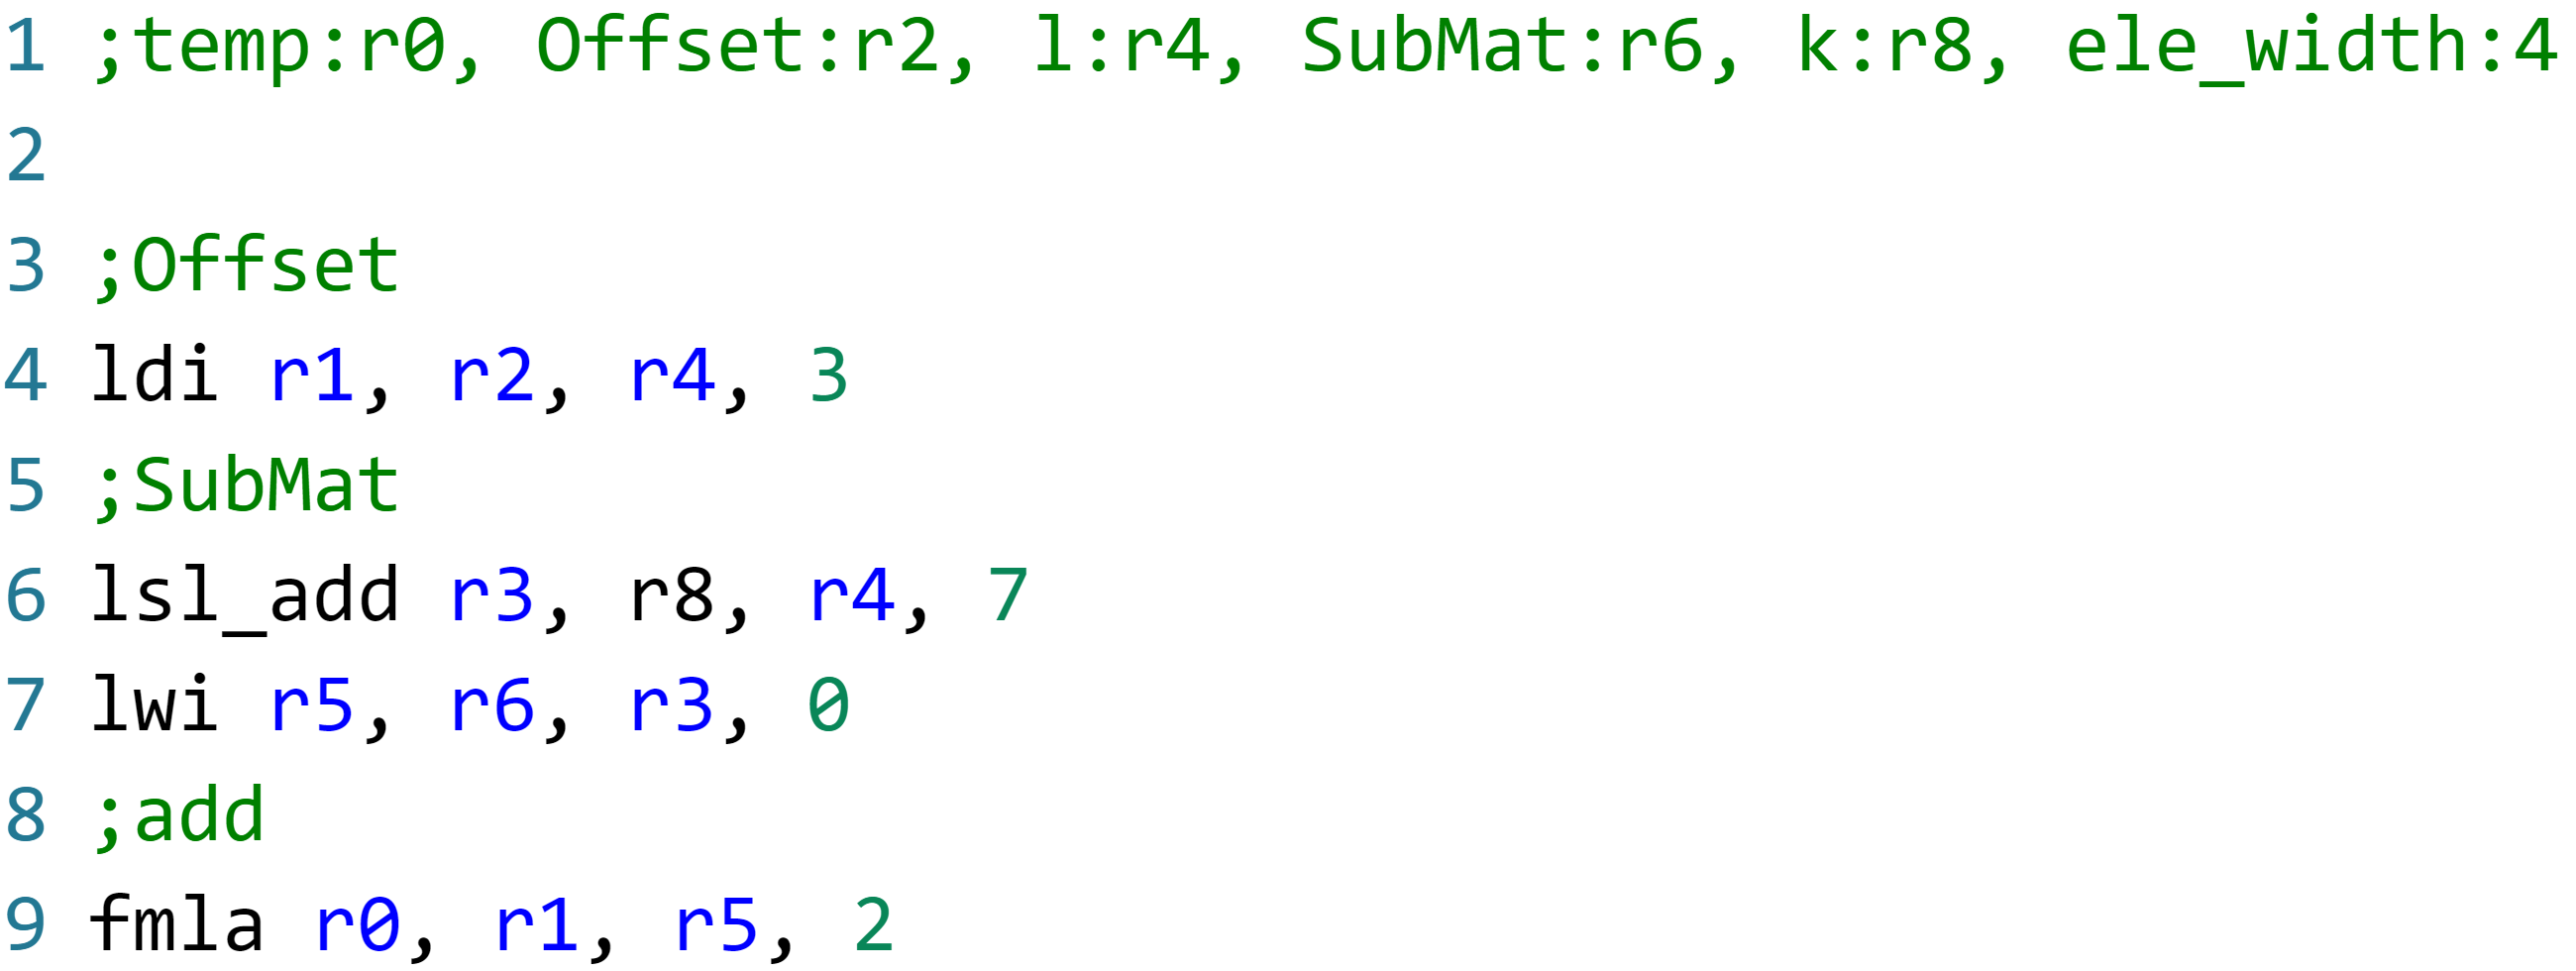
\includegraphics[width=0.3\linewidth]{figures/asm2-opt.png}
        \label{LUTInstAsm:LUT-W-R-opt}}
    \subfigure[LUT-W-C算法优化]{
        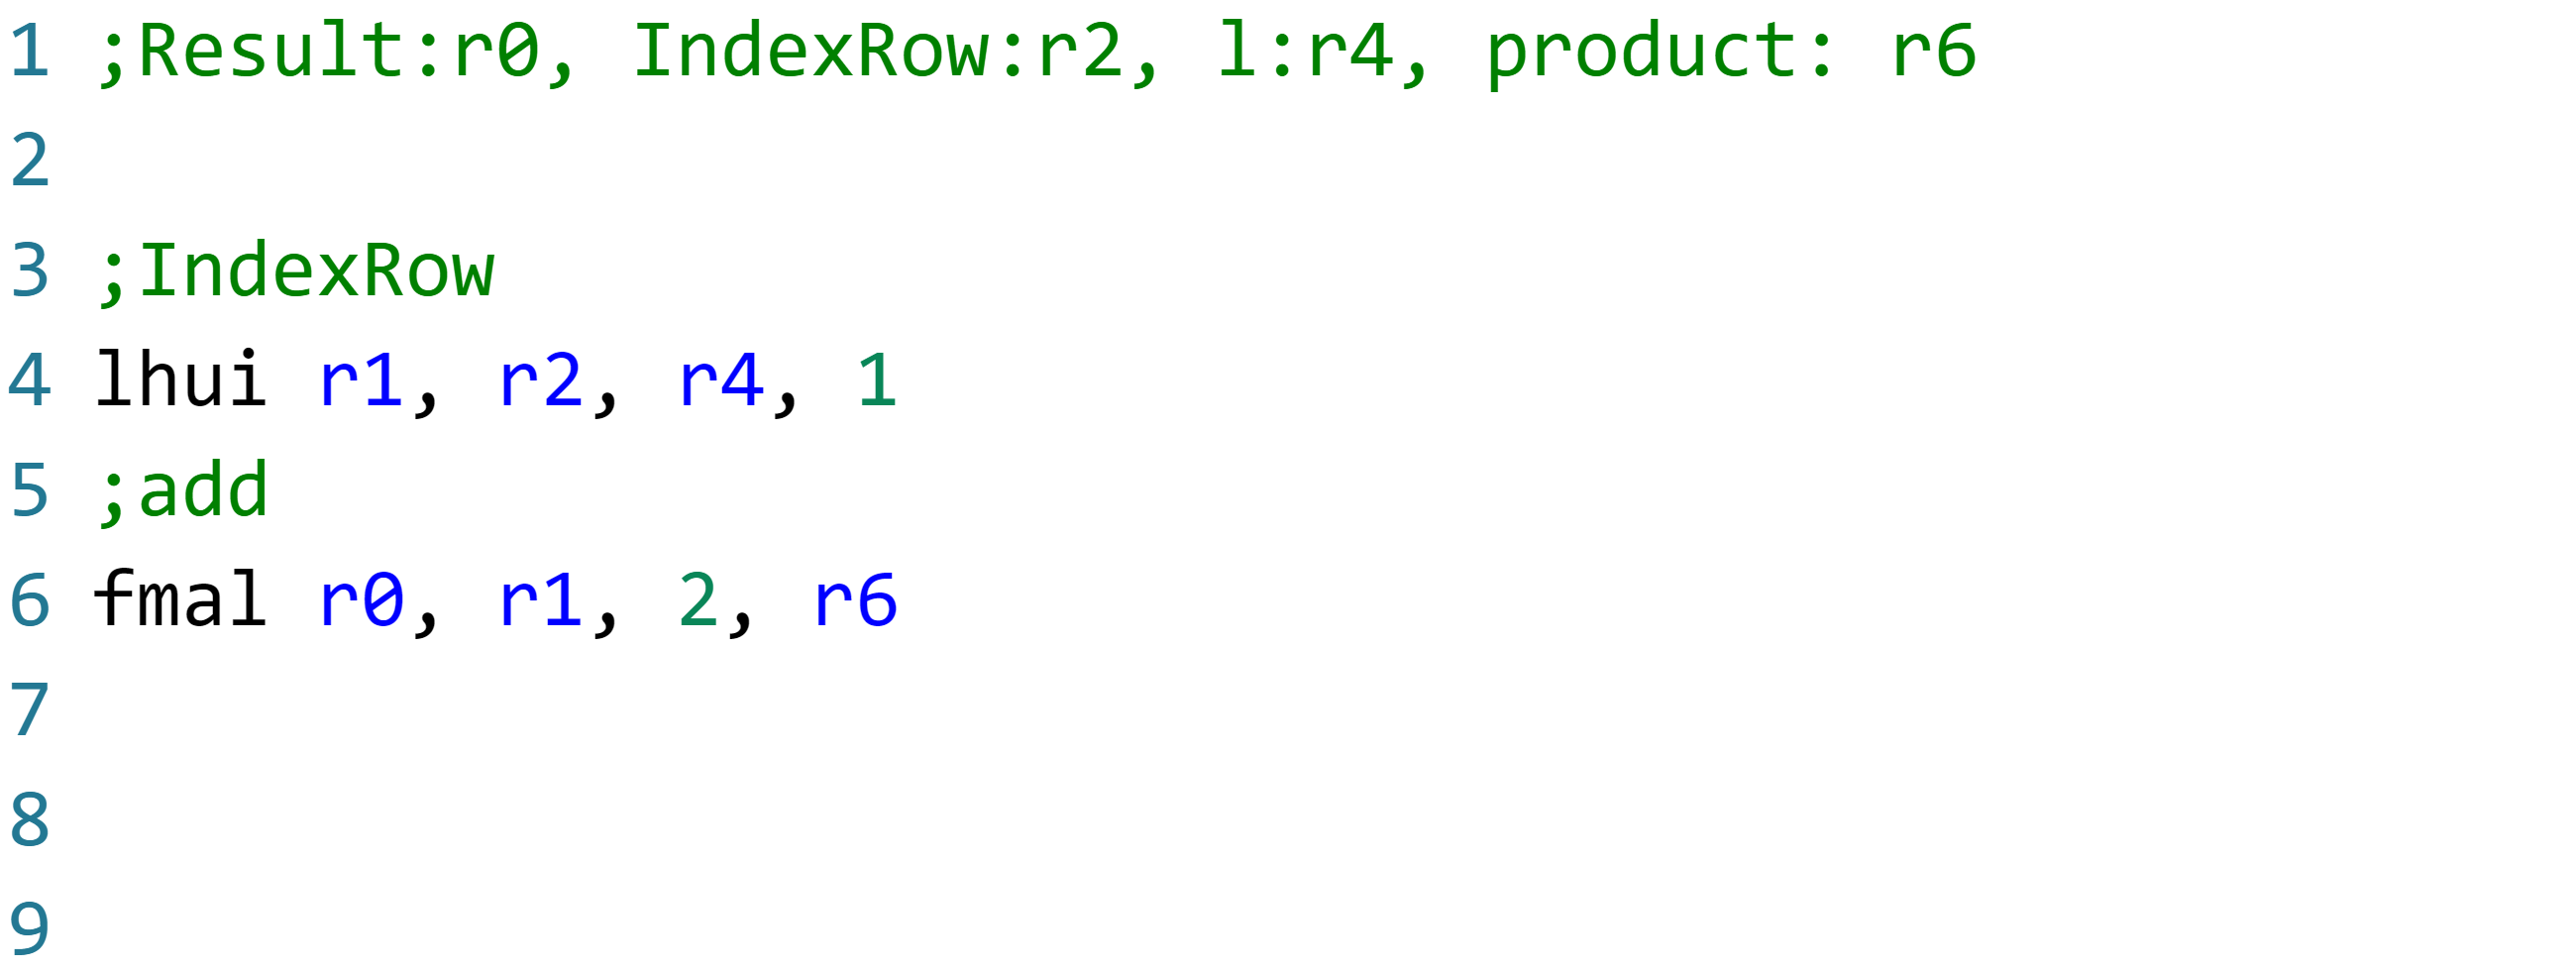
\includegraphics[width=0.3\linewidth]{figures/asm3-opt.png}
        \label{LUTInstAsm:LUT-W-C-opt}}
	\caption{不同GEMV算法查表累加语句汇编分析}
    \label{LUTInstAsm}
\end{figure}

对算法\ref{LUT-M}、\ref{LUT-W-R}、\ref{LUT-W-C}中查表累加语句进行汇编分析:算法LUT-M对应的是\verb|Result[k]+=SubLUT[Vector[j]&0xF][MatRow[k]]|,其编译指令序列如图\ref{LUTInstAsm:LUT-M}所示;算法LUT-W-C对应\verb|Result[IndexRow[l]]+=product|,其指令序列如图\ref{LUTInstAsm:LUT-W-C}所示;算法LUT-W-R对应的是语句\verb|temp+=*(Offset[l]+|     \verb|SubMat[l][k]*ele_width)|,其指令序列如图\ref{LUTInstAsm:LUT-W-R}所示。每做一次数组的访问或者累加操作,至少需要两条甚至以上的指令,现在使用图\ref{LUTInst}中所示的指令集对上述汇编代码进行重写,能够得到优化后的汇编代码如图\ref{LUTInstAsm:LUT-M-opt}、\ref{LUTInstAsm:LUT-W-R-opt}、\ref{LUTInstAsm:LUT-W-C-opt}所示,指令数目大大减少,由原先的6至8条指令减少到2至4条,由2到3倍的提升;由于最深层循环的循环次数是最多的,主要决定程序的性能,因此理论上使用融合查表加法指令能够对程序有2到3倍的性能提升。

\section{基于查表的向量指令设计实现}
SIMD(Single Instruction Multiple Data)是一种特殊的计算模式,即“单指令多数据”,它允许处理器通过一条指令同时对多个数据执行相同的操作,从而显著提高数据处理的效率和性能。在SIMD架构中,处理器执行一条指令,但这条指令会同时作用于多个数据单元,同时执行相同的算术操作,因此SIMD指令非常适用于矩阵和向量的数据计算。Intel是SIMD计算模式的主要推动者之一,为多种架构的处理器配备了SIMD处理单元和对应的指令集\cite{IntelAVX},SIMD的数据位宽从一开始的128bit逐渐增长到256bit最后到512bit,大大提升了数据处理的效率。

\begin{figure}[!htbp]
	\centering
    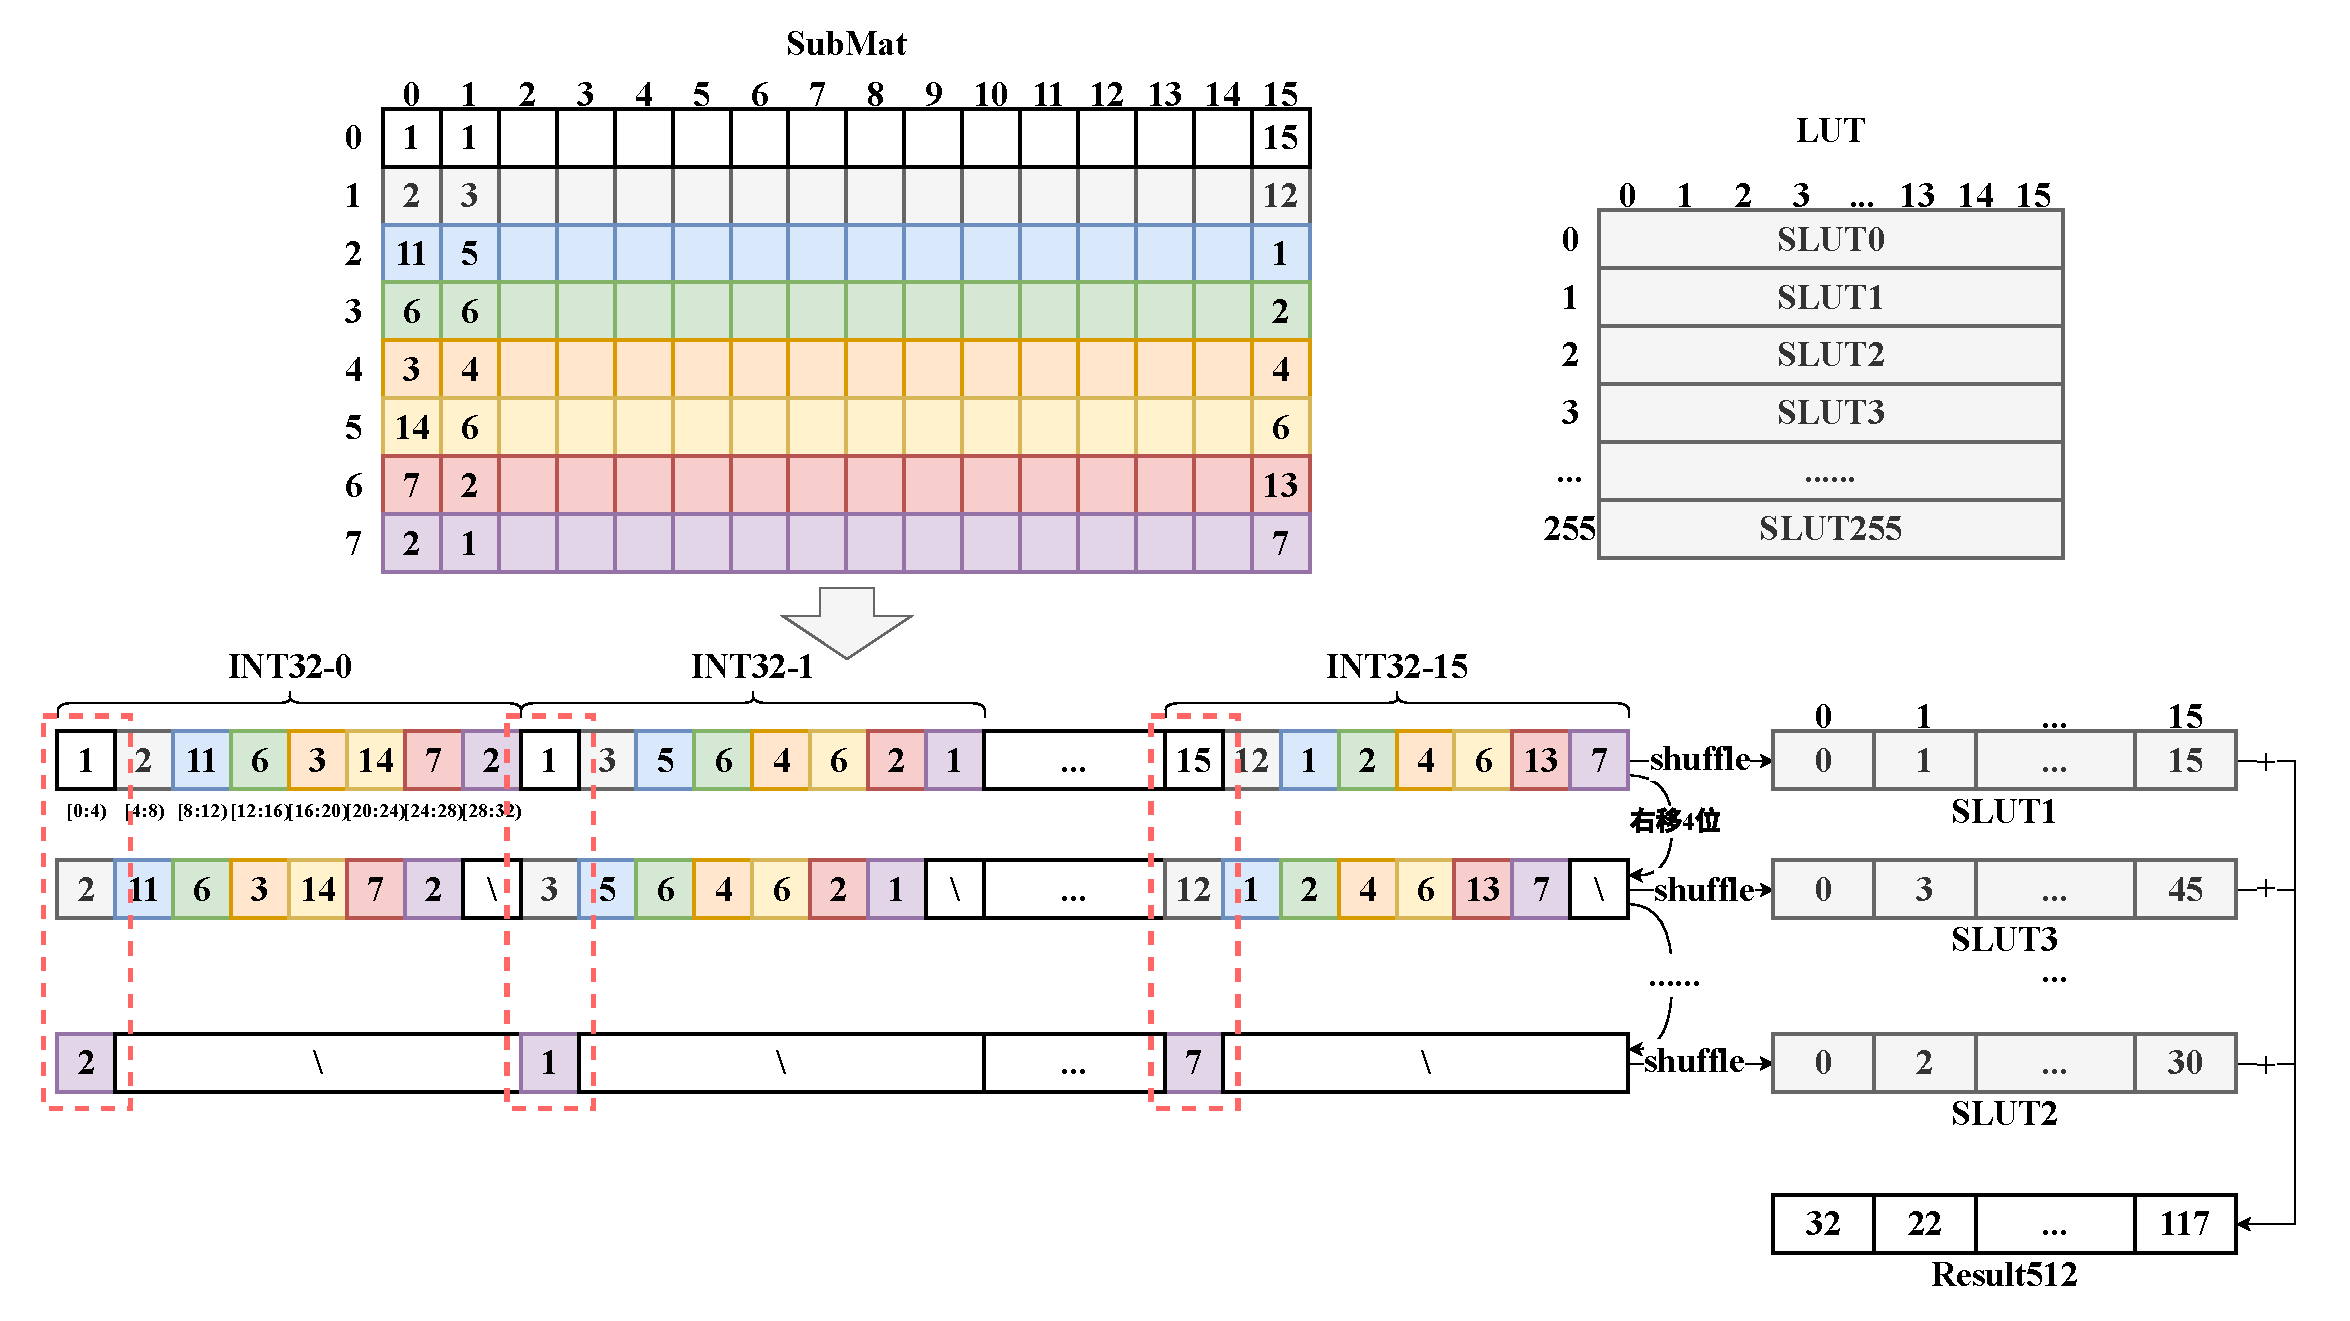
\includegraphics[width=0.9\textwidth]{figures/SIMD.pdf}
	\caption{基于SIMD指令的矩阵构建和GEMV计算}
    \label{SIMD}
\end{figure}

对于更低bit量化,参考Intel AVX向量指令集增添SIMD指令进行加速:\verb|__m512i _mm512_permutexvar_epi32(__m512i idx, __m512i a)|,接受两个AVX-512向量,并返回一个AVX-512向量,这些AVX-512向量由16个32位整型数组成,这个函数的作用是:按照index向量中指示的索引将a向量重排,比如index向量中第1个元素值是3,表示会将a向量中第4个元素重排到新向量的第1个位置。值的注意的是index向量中每个int32只用到了最低4bit的数值(确保索引值不超过16)。这种重排与查表操作存在相同之处,查表本身也是给出一张向量(子查找表),读取权重矩阵元素的值作为索引,再去查找表中取得乘积。上述函数中a向量为子查找表,权重矩阵的一行的前16个元素为index向量,相当于使用权重矩阵的值对子查找表做重排,可以一次性查出16个乘积结果。假设权重矩阵数据宽度为4bit,输入向量仍然是8bit的位宽,那么查找表为$256\times 16$的二维数组,仍然展开FP8到int32,那么LUT的每一行就是一个AVX512向量,刚好满足上述指令的条件。

要想使用SIMD计算GEMV,首先需要对权重矩阵进行重新划分,现以Intel的AVX-512向量为例,对于行主存的矩阵,现将其切分成$8\times 16$的子块SubMat如图\ref{SIMD},对这个子块进行重排,将其转换成一个AVX-512向量:将该AVX-512向量分组,分为16组INT32,将$\text{SubMat[0][0]}$的元素放置到INT32-0的最低四位$[0:4)$,再将$\text{SubMat[1][0]}$的元素放置到INT32-1的$[4:8)$,依次类推,直至遍历完8行,这样就填满了INT32-0,同样的道理,处理SubMat矩阵的第二列,得到INT32-1,当处理完SubMat的所有行和所有列之后,填满了该AVX-512向量。将该向量代替原子矩阵进行存储。完成了所有子块的重排之后,矩阵划分结束,其结果是行数减小到原来的8倍,列数扩大到原来的8倍。这时由于执行的是$8bit\times 4bit$的乘法,查找表的大小为$256\times 16\times 4Byte=16KB$,可以完全载入WRAM,因此可以直接按照GEMV内积的方式计算。

\begin{figure}[!htbp]
	\centering
    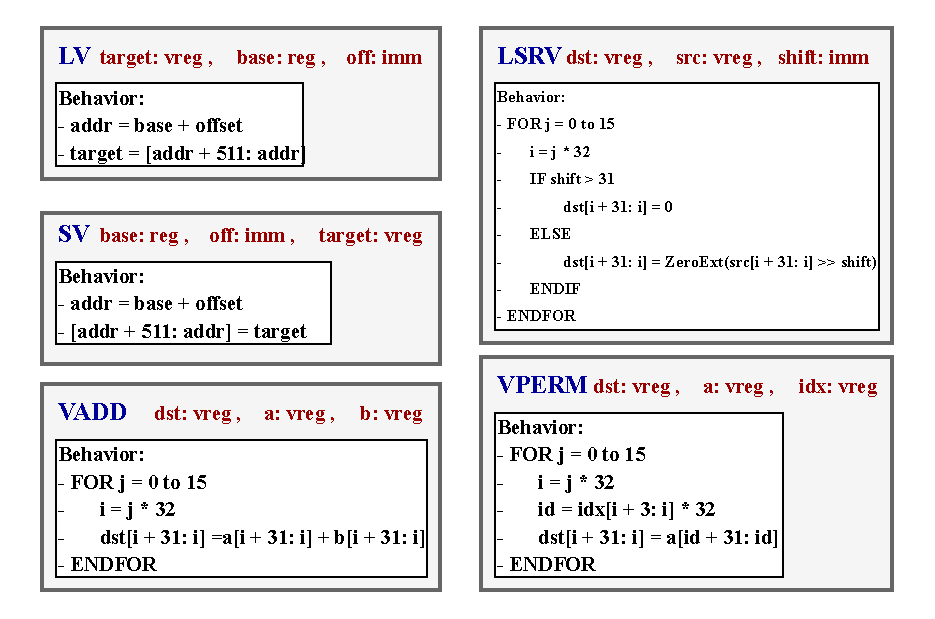
\includegraphics[width=0.9\textwidth]{figures/SIMDInst.pdf}
	\caption{向量指令集设计}
    \label{SIMDInst}
\end{figure}

具体的计算方式也需要将重排后的权重矩阵从行主存改为列主存,也就是以512bit的粒度进行转置。转置过后,原来一列的元素现在可以按照行访问提高访问效率。再基于DPU内部线程并行化,每个tasklet处理一列并均分所有列。具体到单个AVX-512向量,仍然以IntelAVX指令为例,计算仍然以图\ref{SIMD}为例,计算该AVX-512向量时需要先载入对应的子查找表SLUT1到AVX-512向量a中(使用\verb|_mm512_loadu_si512|指令载入寄存器),然后载入权重的AVX-512向量到index寄存器中,执行\verb|_mm512_permutexvar_epi32|操作得到结果,使用\verb|_mm512_add_epi32|指令将其加到AVX-512累加结果寄存器上。然后使用\verb|_mm512_srli_epi32|指令对index向量右移4位,再重复刚才的过程;左移8次后完成整个AVX-512向量的计算,再依次执行该列的所有AVX-512向量的计算,执行完成后再将AVX-512的累加寄存器写到结果向量的对应位置上。不同的tasklet负责不同的列,其对应的结果向量的位置也不同,但是之间互相不干扰无同步开销。

\begin{algorithm}[!htbp]
    \caption{基于SIMD指令的矩阵向量乘算法(LUT-SIMD)}
    \label{LUT-SIMD}
    \begin{algorithmic}[1]
        \Require $Vector[M], TransMat[N/16][M*8], LUT[256][16], MapLUT[256]$; % input
        \Ensure $Result\_8[N]$; % output

        \State $\textbf{define}\;MatBuffer[1024],\;Result\_32[N]$

        \For{$i \gets TaskletId$ \textbf{to} $N / 16 - 1$ \textbf{step} $TaskletNum$}
            \For{$j \gets 0$ \textbf{to} $M * 8 - 1$ \textbf{step} $1024$}
                \State $\textbf{mram\_read}(MatBuffer, \&TransMat[i][j], 1024)$
                \For{$k \gets 0$ \textbf{to} $1023$ \textbf{step} $64$}
                    \State $\textbf{LV}(A, \&MatBuffer[k], 64)$
                    \For{$l \gets 0$ \textbf{to} $7$}
                        \State $\textbf{LV}(Index, LUT[Vector[(j + k) / 8 + l]], 0)$
                        \State $\textbf{VPERM}(Temp, A, Index)$
                        \State $\textbf{VADD}(Adder, Adder, Temp),\quad \textbf{LSRV}(A, A, 4)$
                    \EndFor
                \EndFor
            \EndFor
            \State $\textbf{SV}(\&Result\_32[i*16], 0, Adder)$
        \EndFor

        % 调用二分查找函数
        \State $Result\_8 \gets \textbf{BinarySearch}(Result\_32, MapLUT)$
        \Comment{\textcolor{blue}{parallel in N}}
        \State \Return $Result\_8$
    \end{algorithmic}
\end{algorithm}

要想完成上述工作,需要给UPMEM增加相应的向量单元并适配相应的指令集,如图\ref{SIMDInst}所示,使用LV和SV指令来从内存某处加载/存储512bit的向量到向量寄存器中。使用LSRV指令对512bit向量中的每个32bit数进行右移,右移的位数不超过31位。当然还要使用VADD执行两个512bit向量逐元素加法,以VPERM指令使用index向量对a向量进行重排。同时要高效完成上述工作,每个线程至少需要4个512向量寄存器,其中两个分别充当a和index,剩下的两个一个用于暂存向量重排的结果,一个用作累加寄存器。考虑到硬件实现,由于我们只是支持SIMD的部分计算,仅仅包括重排、加法和位移(向量的Load/Store比较简单),因此向量计算单元的电路设计不会特别复杂,同时由于UPMEM工作特性,线程数量大于11对于性能没有明显提升,存在大量空闲的寄存器(UPMEM有16个物理线程每个线程都有24个32bit寄存器),因此有足够的空间留给向量寄存器堆。

给出基于SIMD向量指令的算法如算法\ref{LUT-SIMD}所示,这里卸载的是$8bit\times 4bit$的乘法,因此查找表的维度是$256\times 16$,刚好可以放进WRAM中且每一行都是一个512bit的向量。权重矩阵需要重排,假设M和N都为4096,原本的维度是$4096\times 4096$,使用int8存储数组的维度是$4096\times 2048$,重排之后行缩小8倍,列扩大8倍变为$512\times 16384$,再按照512bit(64B)的粒度进行行列转置,维度就变成$256\times 32768$。上述操作中最深层循环的操作是指令LV、VPERM和VADD,每次执行这三条指令就可以一次性对16个数进行查表并累加,大大提升了性能。

\section{基于近存模拟器的硬件设计实现}
为了实现上述硬件的修改并验证性能,需要使用一个能够模仿UPMEM硬件计算的软件。PIMulator是一个UPMEM的周期精确模拟器\cite{uPimulator},能够满足我们修改硬件的需求。它由两个关键组件组成,如图\ref{PIMulator}所示:一个是与UPMEM指令集架构(Instruction Set Architecture, ISA)兼容的软件编译工具链,以及一个经过真实UPMEM-PIM硬件交叉验证的硬件性能模拟器。

PIMulator的软件编译工具链的一部分基于开源的UPMEM软件开发工具包\footnote{https://sdk.upmem.com}(Software Development Kit,SDK)提供的LLVM\cite{LLVM}编译器工具链(dpu-upmem-dpurte-clang),另一部分包括自定义的编译器、链接器和汇编器。PIMulator主要是用UPMEM SDK提供的编译器将用户所书写的能在真实硬件上运行的源代码以及和UPMEM兼容的C标准库程序进行预处理、编译和汇编成二进制对象,最终链接形成UPMEM的可执行二进制文件。同时,PIMulator使用自定义设计的链接器和汇编器,而不是直接使用UPMEM SDK的链接器。这是因为UPMEM的链接器与UPMEM硬件的微架构紧密绑定,限制了对PIM硬件架构的自定义能力。例如,当编译后的程序大小或WRAM内存使用量超过物理IRAM或WRAM容量时,UPMEM的链接器会报错。

\begin{figure}[!htbp]
	\centering
    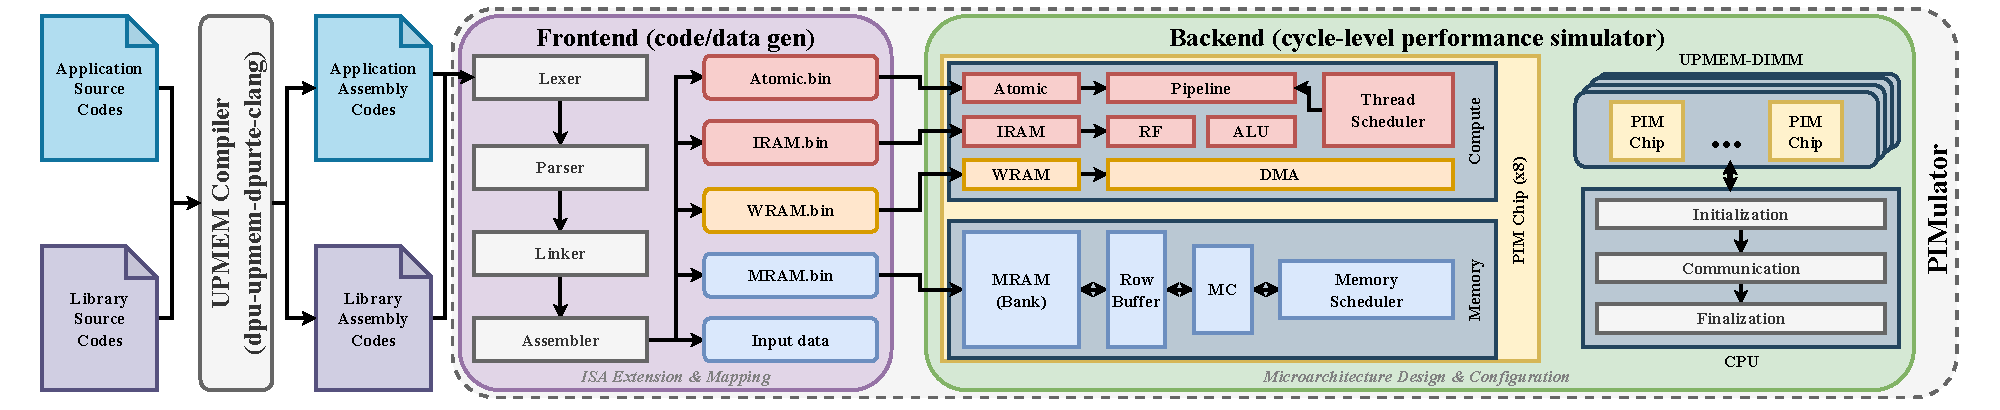
\includegraphics[width=0.9\textwidth]{figures/PIMulator.pdf}
	\caption[PIMulator架构图]{PIMulator架构图,重绘自文章\cite{uPimulator}}
    \label{PIMulator}
\end{figure}

PIMulator的硬件周期精确模拟器设计参考了UPMEM的用户手册和公开的微架构信息,主要设计点包括:1)对DPU计算核心进行建模:DPU核心被建模为一个14级顺序流水线处理器,充分模拟了流水线的调度算法以及奇偶寄存器堆访问时的限制。2)DRAM子系统建模:PIMulator的DRAM子系统模拟基于GPGPU-Sim的周期级DRAM模拟\cite{GPGPU-Sim}。由于UPMEM-PIM的内存调度策略细节未公开,PIMulator采用了首行优先,先到先服务(First Row, First Come First Served,FR-FCFS)算法来调度内存事务。3)CPU-DPU通信:设定固定通信值来模拟CPU和DPU之间的通信延迟,其值通过UPMEM-PIM真实硬件的系统性的性能分析来调整。UPMEM使用Intel AVX指令进行CPU-DPU通信,PIMulator同样模拟了这种通信的不对称带宽特性。

PIMulator有多个版本的实现\footnote{https://github.com/VIA-Research/uPIMulator},在论文中实现的是前后端分离的单线程版,使用Python实现前端,C++做硬件模拟后端,没有多线程支持,平均模拟速率为3KIPS(千条指令每秒),与GPGPU-Sim相当。PIMulator另有一版基于Golang开发的前后端一体的版本,充分利用多协程(coroutine)实现了模拟速度提8.5倍的提升并且内存占用减少7.5倍。

PIMulator的设计采用了模块化结构,将SPMD的前端代码/数据生成与后端模拟器清晰分离,类似于GPGPU-Sim的设计。这种设计使得PIMulator可以轻松扩展以模拟和评估新的软硬件架构。本文的硬件架构改动使用PIMulator的这种前后端分离架构实现,具体来说对于改动一的新增的融合查表加法单元,在定义好指令的格式后,会在前端直接修改GEMV算子的汇编代码并使用自定义的FLA指令集,然后修改前端汇编器,包括语法分析和词法分析的程序,使得前端程序能够正确识别我们新增的指令。与此同时,在后端的逻辑部分新增对应指令的逻辑计算,以函数的形式暴露给后端模拟仿真,就相当于增添了相应的硬件单元。对于改动二SIMD指令也是类似的流程,不过稍有不同之处在于SIMD指令需要自行添加向量寄存器并识别,这个需要在前后端的寄存文件中去定义向量寄存器。

\section{本章小结}
本章主要介绍了在近存计算模拟器上修改硬件加速矩阵向量乘的设计。首先对此前提出的软件算法进行了分析,分析算子的性能瓶颈在于商用硬件的计算性能上,阐明了修改硬件的原因和必要性。接着介绍了设计的融合查表加法指令集,通过对矩阵乘法汇编代码的分析和比较表明引入该融合查表加法指令会大幅减少指令数目并加速程序。然后是对UPMEM增加向量单元的设计,详细描述了权重矩阵的重排流程、SIMD指令集的设计和基于向量指令的GEMV算法,通过向量化访存和计算能够极大提高程序效率。最后介绍了上述硬件改动的实现,包括模拟器平台PIMulator的介绍和修改方式。